

\input{"C:/Users/spileggi/Google Drive/STAT 330/Lectures/SlideStyle.tex"}



\title[Lecture 2]{Introduction to SAS Procedures}
\author[Pileggi]{Shannon Pileggi}

\institute[STAT 330]{STAT 330}

\date{}


\begin{document}

\begin{frame}
\titlepage
\end{frame}

\begin{frame}
\frametitle{OUTLINE\qquad\qquad\qquad} \tableofcontents[hideallsubsections]
\end{frame}



%===========================================================================================================================
\section[Programming Basics]{Programming Basics}
%===========================================================================================================================

\subsection{}
\begin{frame}
\ft{Programming Tips}
\begin{enumerate}
    \item Create a `game plan' before you start programming
    \bi
    \item this can be a mental list OR a plain English description of your plan (or pictures or diagrams - whatever you find most helpful)
    \item this step is not required, but can save you hours of wasted time!
    \item if you get stuck and ask for help, I will most likely ask you about your `game plan'
    \item[]
    \ei
    \item Don't try to program the entire thing at once
    \bi
    \item work on one part at a time
    \item if you spend more than an hour on something and you are still unable to figure it out, you should ask for help
    \ei
\end{enumerate}
\end{frame}

\begin{frame}[fragile]
\frametitle{SAS programs}
\begin{center}
A SAS program is executed \\
\vskip5pt
\emph{line by line} \\
\vskip5pt
and \\
\vskip5pt
\emph{observation by observation}.\\
\end{center}
\begin{clicker}{Which of the following pseudo-code chunks would successfully create $Z$ as the product of $X$ and $Y$?}
\bmp{0.10\textwidth}
\hspace{1in}
\emp
\bmp{0.30\textwidth}
\begin{craw}{.0}{Program 1}
z =  x * y ;
x = 5 ;
y = 3 ;
\end{craw}
\emp
\bmp{0.10\textwidth}
\hspace{1in}
\emp
\bmp{0.30\textwidth}
\begin{craw}{.0}{Program 2}
x = 5 ;
y = 3 ;
z =  x * y ;
\end{craw}
\emp
\end{clicker}
%\bi
%\item[]
%\item SAS executes line 1 of your data before it executes line 2
%\item So if \ttb{\ttu{Z=X*Y}}, then make sure that statements creating \ttb{\ttu{X}} and \ttb{\ttu{Y}} come before the statement creating \ttb{\ttu{Z}}.
%\ei
\end{frame}


\begin{frame}
\ft{Errors and debugging}
Common Errors:
\bi
\item Statements that are out of order
\item Misspelling a variable name or SAS key word
\item Forgetting a semi-colon
\item Not closing a comment or quote
\item Not highlighting an entire DATA or PROC step and submitting it
\item[]
\ei
Debugging methods:
\bi
\item Check your log
\item Use comments to stepwise hide/reveal your code until you identify the error
\item Submit a single quote,or semi-colon, or \ttt{run;} by itself
\item Save your code, \ttb{exit} SAS, and re-launch SAS to start from a clean slate.
\ei
\end{frame}

%===========================================================================================================================
\section[PROC CONTENTS]{PROC CONTENTS}
%===========================================================================================================================
\subsection{}
\begin{frame}
\tableofcontents[currentsection, hideallsubsections]
\end{frame}

\begin{frame}[fragile]
\ft{\ttt{PROC CONTENTS}}
\bmp{1.0\textwidth}
\footnotesize
\begin{code}{.0}
PROC CONTENTS DATA = sashelp.cars;
RUN;
\end{code}
\emp
\vskip10pt
\begin{itemize}
    \item \ttt{PROC CONTENTS} displays information about the SAS data set
    \bi
    \item data set name, number of observations, number of variables, date created
    \item for each variable: type, length, formats, and informats
    \ei
    \item By default, variables are listed in alphabetical order
    \item When working with a new data set, always use \ttt{PROC CONTENTS} first!
\end{itemize}
\end{frame}

\begin{frame}
\ft{Labels and formats}
Labels
\begin{itemize}
\item Variable names are typically short, but sometimes not informative
\item Use \ttb{labels} to replace variables names in output
\item Labels can be up to 256 characters long
\item[]
\end{itemize}
Formats
\begin{itemize}
\item Variable \emph{values} may not always be displayed in an easy to read manner (eg, SAS dates, money)
\item \ttb{Formats} to change the display of variable values in output
\end{itemize}
\end{frame}

\begin{frame}[fragile]
\ft{Working with PROCS}
All PROCS have \emph{required} and \textcolor{OrangeRed}{\emph{optional}} statements.
\vskip10pt
\bmp{1.0\textwidth}
\footnotesize
\begin{code}{.0}
PROC CONTENTS DATA = sashelp.cars \textcolor{OrangeRed}{VARNUM};
RUN;
\end{code}
\emp
\vskip20pt
Here, \textcolor{OrangeRed}{\ttt{VARNUM}} is actually an \textcolor{OrangeRed}{\emph{optional}} statement.  To see all optional statements, examine the help file for that procedure.
\vskip20pt
\oyo Examine the help file for \ttt{PROC CONTENTS} to determine what \textcolor{OrangeRed}{\ttt{VARNUM}} does.
\end{frame}

\begin{frame}[fragile]
\ft{Titles}
\begin{code}{.0}
title "Contents of cars data, alphabetical variables";
PROC CONTENTS DATA=sashelp.cars;
RUN;
title;
\end{code}
\vskip10pt
Title statements
\bi
\item can be \emph{inside} or \emph{outside} the \ttt{PROC}.
\item will \textbf{carry through} for all future output.
\item can be turned off by submitting \fbox{\ttt{title;}}.
\ei
\end{frame}

%===========================================================================================================================
\section[PROC PRINT]{PROC PRINT}
%===========================================================================================================================
\subsection{}
\begin{frame}
\tableofcontents[currentsection, hideallsubsections]
\end{frame}

\begin{frame}[fragile]
\ft{\ttt{PROC PRINT}}
\bmp{1.0\textwidth}
\footnotesize
\begin{code}{.0}
PROC PRINT DATA = sashelp.cars;
RUN;
\end{code}
\emp
\vskip10pt
\begin{itemize}
    \item \ttt{PROC PRINT} displays values of the SAS data set
    \item By default, all observations and variables are printed
\end{itemize}
\end{frame}

\begin{frame}[fragile]
\ft{\ttt{PROC PRINT}, optional statements}
\bmp{1.0\textwidth}
\footnotesize
\begin{code}{.0}
PROC PRINT DATA = sashelp.cars (OBS=10);
	VAR msrp enginesize;
RUN;
\end{code}
\emp
\vskip20pt
\oyo Predict what this will do before you submit it.
\end{frame}



\begin{frame}[fragile]
\ft{\ttt{PROC PRINT}, optional statements}
\bmp{1.0\textwidth}
\footnotesize
\begin{code}{.0}
PROC PRINT DATA = sashelp.cars (OBS=10) \textcolor{OrangeRed}{\underline{\hspace{0.5in}}};
	VAR make model msrp enginesize;
RUN;
\end{code}
\emp
\vskip20pt
\oyo Use the help file for \ttt{PROC PRINT} to replace the blank with an option to display the variable label rather than the variable name as shown in the partial output.
%label key word
\vskip10pt
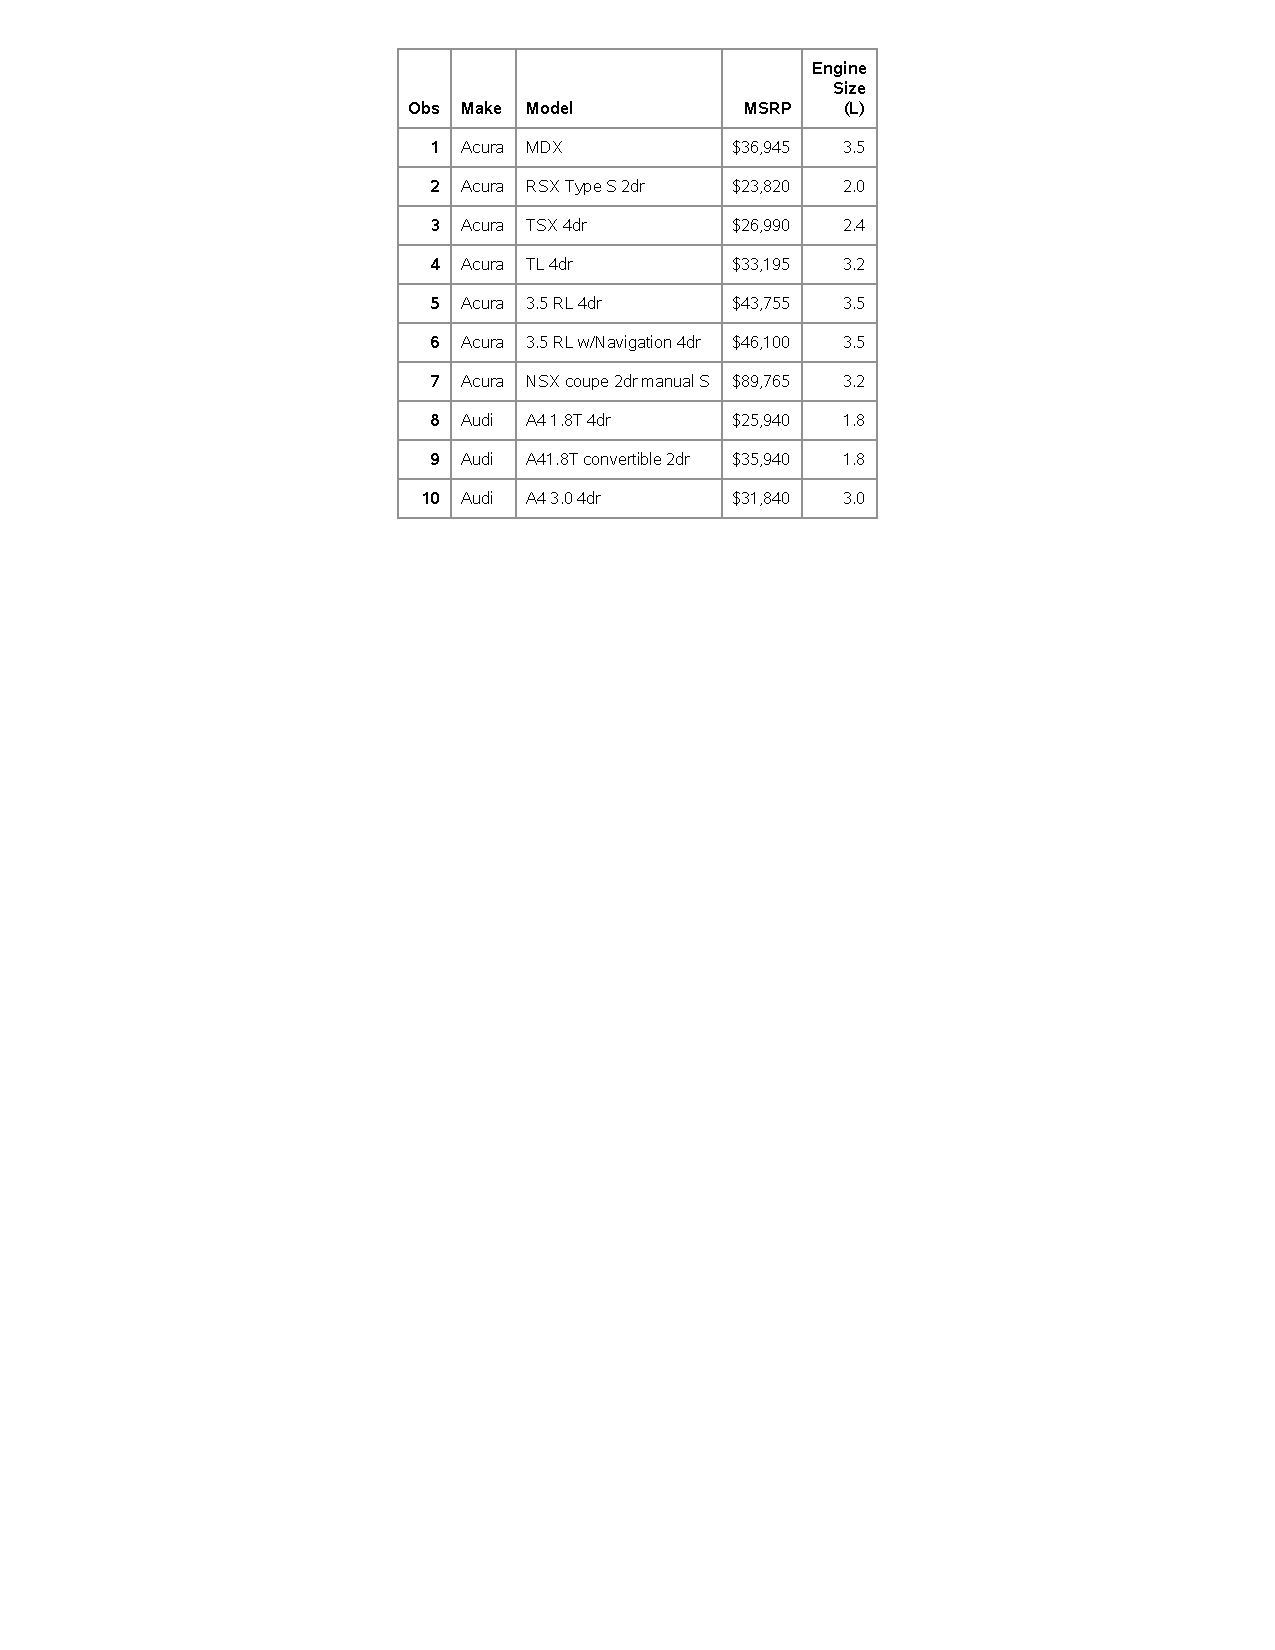
\includegraphics[trim={5cm 20cm 5cm 0.5cm},clip,width=0.8\textwidth]{L2_procprint.pdf}
\end{frame}



\begin{frame}
\ft{More options in \ttt{PROC PRINT}}
\bi
\item \ttt{NOOBS} - suppresses observation numbers
\item \ttt{LABEL} or \ttt{L} - Uses labels instead of variable names
\item \ttt{BY var\_1 var\_2 ... var\_k}
	\bi
	\item will start a new section for the different values of the specified
variable(s); data \tte{must} already be sorted according to the \ttt{BY} variables (see \ttt{PROC SORT}).
	\ei
\item \ttt{ID var\_1 var\_2 ... var\_k}
	\bi
	\item Observation numbers are omitted, ID variable value is included instead
	\ei
\item \ttt{VAR var\_1 var\_2 ... var\_k}
	\bi
	\item specifies which variables to print
	\ei
\item \ttt{SUM var\_1 var\_2 ... var\_k}
	\bi
	\item prints sums for specified numeric variables
	\ei
\ei
\end{frame}

%===========================================================================================================================
\section[PROC MEANS]{PROC MEANS}
%===========================================================================================================================
\subsection{}
\begin{frame}
\tableofcontents[currentsection, hideallsubsections]
\end{frame}


\begin{frame}[fragile]
\ft{\ttt{PROC MEANS}}
\bmp{1.0\textwidth}
\footnotesize
\begin{code}{.0}
PROC MEANS DATA = sashelp.cars;
RUN;
\end{code}
\emp
\vskip10pt
\begin{itemize}
    \item \ttt{PROC MEANS} produces basic summary statistics 
    \item By default, $N$, mean, sd, min, and max are calculated for all \emph{numeric} variables
\end{itemize}
\end{frame}


\begin{frame}[fragile]
\ft{\ttt{PROC MEANS}, optional statements}
\bmp{1.0\textwidth}
\footnotesize
\begin{code}{.0}
PROC MEANS DATA = sashelp.cars ;
	VAR msrp enginesize;
RUN;
\end{code}
\emp
\vskip20pt
\oyo Predict what this will do before you submit it.
\end{frame}

\begin{frame}[fragile]
\ft{\ttt{PROC MEANS}, optional statements}
\bmp{1.0\textwidth}
\footnotesize
\begin{code}{.0}
PROC MEANS DATA = sashelp.cars ;
	VAR make model msrp enginesize;
RUN;
\end{code}
\emp
\vskip20pt
\oyo Predict what this will do before you submit it.
\end{frame}

\begin{frame}[fragile]
\ft{\ttt{PROC MEANS}, optional statements}
\bmp{1.0\textwidth}
\footnotesize
\begin{code}{.0}
PROC MEANS DATA = sashelp.cars (OBS=10) \textcolor{OrangeRed}{\underline{\hspace{0.5in}}};
	VAR msrp enginesize;
RUN;
\end{code}
\emp
\vskip20pt
\begin{columns}
\column{0.55\textwidth}
\oyo Use the help file for \ttt{PROC MEANS} to replace the blank with \emph{options} to display only the mean rounded to two decimal places as shown.
\column{0.40\textwidth}
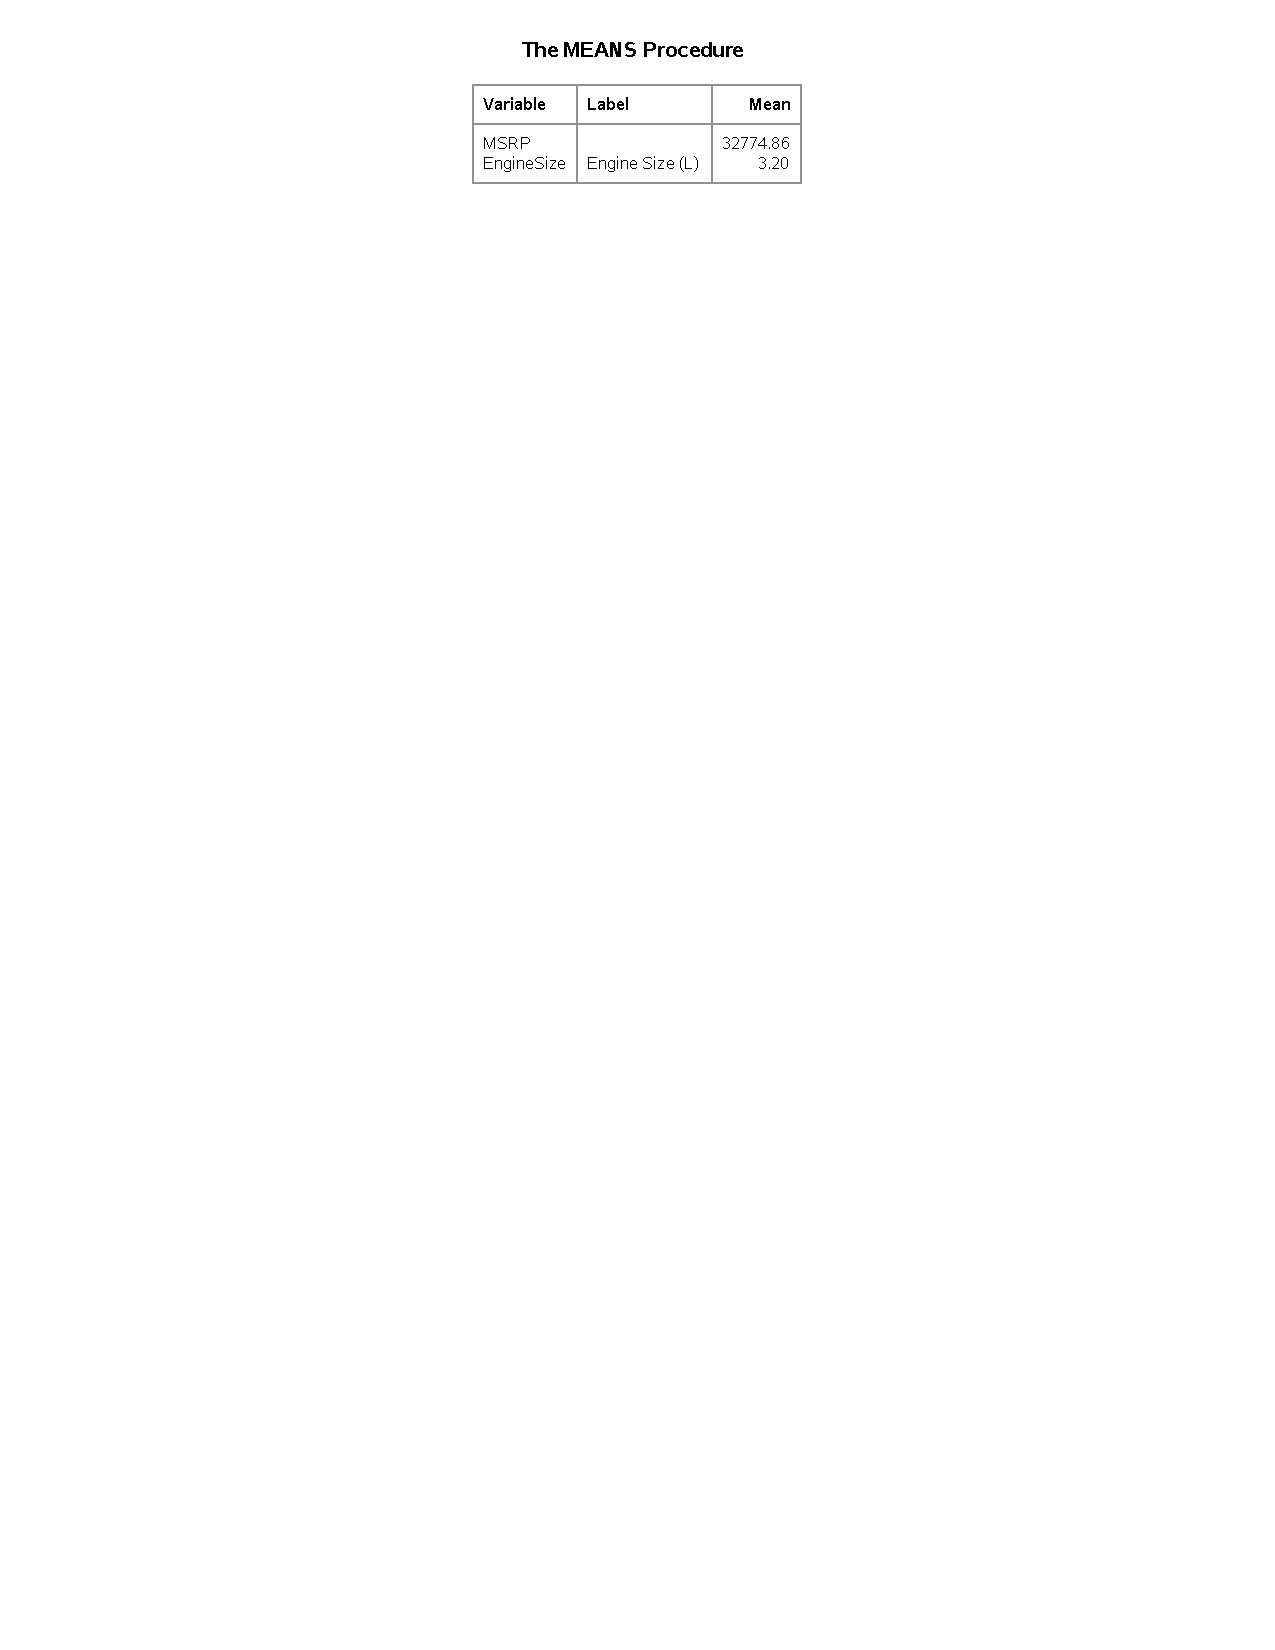
\includegraphics[trim={8.0cm 24.5cm 8cm 1.3cm},clip,width=1.0\textwidth]{L2_procmeans.pdf}
\end{columns}
%maxdec=2 mean
\end{frame}

\begin{frame}
\ft{More options in \ttt{PROC MEANS}}
\bi
    \item the \ttt{CLASS} statement defines subgroups for analysis 
    \bi
        \item think results separated by a categorical variable, but condensed on a single page
    \ei 
    \item[]
    \item the \ttt{BY} produces separate results by subgroups for analysis
    \bi 
        \item think results separated by a categorical variable, but separated in multiple tables
        \item requires data to be sorted prior to execution
    \ei 
\ei 
\end{frame}

%===========================================================================================================================
\section[PROC IMPORT]{PROC IMPORT}
%===========================================================================================================================
\subsection{}
\begin{frame}
\tableofcontents[currentsection, hideallsubsections]
\end{frame}

\begin{frame}[fragile]
\ft{PROC IMPORT}
\bmp{1.0\textwidth}
\footnotesize
\begin{code}{.0}
PROC IMPORT
   DATAFILE = "\emph{Computer Location/mydata.ext}"
   OUT = \emph{DataSetName}
   DBMS = \emph{identifier}
   REPLACE ;
RUN;
\end{code}
\emp
\vskip10pt
\bmp{0.10\textwidth} \hspace{0.05in} \emp
\bmp{0.90\textwidth}
\bi
\item[\fbox{\ttt{DATAFILE=}}] takes computer location, data file name, and extension of the data file
\item[\fbox{\ttt{OUT=}}] specifies the SAS data set name you want to create
\item[\fbox{\ttt{DBMS=}}] specifies type of data (e.g., \ttt{CSV}, \ttt{TAB}, \ttt{DLM})
\item[\fbox{\ttt{REPLACE}}] option overwrites an existing SAS data set called \emph{DataSetName}
\ei
\emp
\end{frame}


\begin{frame}
\frametitle{The American Community Survey (ACS)}
\begin{itemize}
    \item
    Each year since 2005, the U.S. Census Bureau has surveyed about 3.5 million households with the American Community Survey (ACS) \url{http://www.census.gov/programs-surveys/acs/}
    \item
    The data are used in government and policy decisions, and helps to determine the allocation of more than \textbf{\$400 billion} in federal and state funds each year.
    \item In the spring of 2012 the House of Representatives voted to eliminate the survey.  Daniel Webster (R):
        \begin{itemize}
        \item
        \emph{This is a program that intrudes on people’s lives, just like the Environmental Protection Agency or the bank regulators.}
        \item
        \emph{We’re spending \$70 per person to fill this out. That’s just not cost effective}.
        \item
        \emph{In the end, this is not a scientific survey. It’s a random survey.}
    \end{itemize}
        \item
    Senator Rand Paul sponsored a \href{http://www.govtrack.us/congress/bills/112/s3079}{bill} to make participation in the ACS voluntary.
\end{itemize}
\end{frame}

\begin{frame}[fragile]
\ft{The data}
\hspace*{-0.3in}
\bmp{1.13\textwidth}
\footnotesize
\begin{craw}{.0}{first few rows of acs.csv}
Sex,Age,MarStat,Income,HoursWk,Race,USCitizen,HealthInsurance,Language
female,31,not married,60,40,white,citizen,yes,other
male,31,not married,0.36,12,black,citizen,yes,native English
male,75,not married,0,,white,citizen,yes,native English
female,80,not married,0,,white,citizen,yes,native English
\end{craw}
\emp
\vskip20pt
\oyo What features do you see in the data that might need to be addressed to import it?
\vskip15pt
\emph{Note:} A data file \underline{\ttb{cannot}} be open in Excel when you try to import it into SAS.
\end{frame}

\begin{frame}[fragile]
%\ft{Importing the data}
\bmp{1.0\textwidth}
\footnotesize
\begin{code}{.0}
PROC IMPORT \textcolor{OrangeRed}{\fbox{\ttt{1}}}
   DATAFILE="X:/StatStudio/spileggi/Data Sets/acs.csv" \textcolor{OrangeRed}{\fbox{\ttt{2}}}
   OUT = acs \textcolor{OrangeRed}{\fbox{\ttt{3}}}
   DBMS = CSV \textcolor{OrangeRed}{\fbox{\ttt{4}}}
   REPLACE \textcolor{OrangeRed}{\fbox{\ttt{5}}}
RUN;
\end{code}
\emp
\vskip10pt
\oyo
\begin{enumerate}
\item Which numbered locations require a semi-colon?
\item Why is the \ttt{REPLACE} option useful?
\item Did we need to address any of the features we discussed?
\item Briefly compare the data in SAS to the data in the CSV file.  What differences do you notice?
%noncitizen
\end{enumerate}
\end{frame}

\begin{frame}[fragile]
\ft{GUESSINGROWS}
\bi
\item \ttt{GUESSINGROWS} specifies the number of rows to scan to determine the appropriate \emph{type} and \emph{length} for variables
\item the default value is 20
\item \oyo What value of \ttt{GUESSINGROWS} do you recommend to correctly import the data?
%163

\ei
\vskip10pt
\bmp{0.9\textwidth}
\footnotesize
\begin{code}{.0}
PROC IMPORT
   DATAFILE="X:/StatStudio/spileggi/Data Sets/acs.csv" 
   OUT = acs
   DBMS = CSV
   REPLACE ;
   \underline{GUESSINGROWS=\textcolor{OrangeRed}{?};}
RUN;
\end{code}
\emp
\end{frame}

\begin{frame}
\ft{The Import Wizard}
\bi
\item \ttt{File -> Import Data}
\item \ttt{Select data source -> Next}
\item \ttt{Browse -> } for file location \ttt{-> Next}
\item \ttt{Library -> WORK}, \ttt{Member:} \emph{DataSetName} \ttt{-> Next}
\item \ttt{Browse -> } create \ttt{.sas} file that saves \ttt{PROC IMPORT} code
\item \ttt{-> Finish}
\ei
\end{frame}

\begin{frame}[fragile]
\ft{Code generated by the import wizard}
\hspace*{-0.25in}
\bmp{1.1\textwidth}
\footnotesize
\begin{code}{.0}
PROC IMPORT
   OUT= WORK.ACS
   DATAFILE= "X:/StatStudio/spileggi/Data Sets/acs.csv" 
   DBMS=CSV REPLACE;
   GETNAMES=YES;
   DATAROW=2;
RUN;
\end{code}
\emp
\vskip15pt
\oyo What would you need to change about this code in order to correctly import the data?
\end{frame}


\end{document} 